\section{Funksjonsanalyse: FAST}
\label{sec:fast}

\subsection{FAST - intro}

FAST står for Function Analisys System Technique, og er en funksjonsanalyse som kan inngå som en del av en systemanalyse. Ved å bruke FAST får vi fram sammenhengen mellom funksjoner, og vi ser hvilke som er avhengig av hverandre. FAST kan også brukes for å samle et team om en idé og sørge for at alle er på samme banehalvdel.


Det mest sentrale konseptet i FAST-teknikken er hvorfor/hvordan-spørsmålet. Ved å stille dette spørsmålet til funksjonene vi har listet opp, får vi kausal-oversikt i systemet.

FAST-teknikken kommer fra feltet Value Engineering, som handler om å skape samme funksjon for mindre kostnad. Dette egner FAST seg spesielt for ettersom metoden identifiserer funksjoner og sammenhenger som gjør det lett å bytte ut funksjoner for å oppnå samme mål.


\subsection{Metode}

FAST gjøres best i team. For å sette i gang kreativiteten, gjør man gjerne en systemdekomponering og lister opp komponentenes funksjoner, før man går videre og setter disse opp i et "hvorfor/hvordan"-diagram. Deretter kan man sette disse sammen i et fullstendig FAST-diagram.

\textbf{Funksjonens navn}: Funksjonens navn spiller en viktig rolle i FAST og det er fafstsatte konvensjoner for hvordan man skal navngi funksjoner. Dette er for å sikre at man er spesifikk nok, og for å sette i gang kreativiteten.
Fuksjonsnavnet skal umiddelbart si noe om formålet bak funksjonen, uten å nødvendigvis si noe om metoden for å gjøre det. Hovedregelen er at funksjoner skal starte med et aktivt verb og avslutte med et substantiv. Eksempler:

\begin{itemize}
    \item Lad batteri
    \item Klipp gress
\end{itemize}

Eksempel på FAST-diagram for ankermekanisme på båt:

\begin{figure}[H]
    \centering
        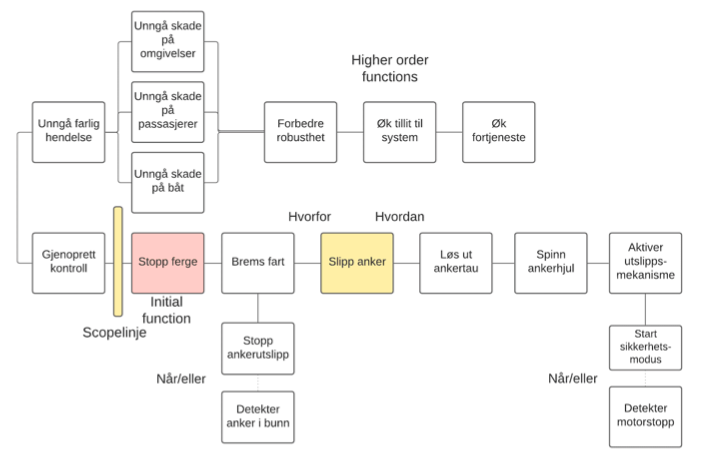
\includegraphics[width=\textwidth]{figures/FAST/Skjermbilde 2021-11-24 kl. 09.28.51.png}\\
        \caption{FAST-diagram for ankermekanisme på båt.}
\end{figure}

Vi ser at i dette FAST-diagrammet er det også gjort litt videre analyse enn bare hvorfor/hvordan. Her er det også lagt inn en såkalt "scopelinje", som er en linje som markerer primærbehovet for mekanismen, det vil si hovedoppgaven til systemet. Scopelinjen settes der hvor man kan si at "dersom funksjonen til høyre for linjen ikke hadde vært der, hadde vi ikke hatt behov for noen av de andre funksjonene heller", også kalt "initial function". I dette tilfellet kan vi se at dette er "Stopp Ferge", som blir hovegrunnen til at vi lnsker å implementere ankermekanismen. Dersom vi ikke ønsket å stoppe fergen, hadde vi f. eks. heller ikke trengt å bremse farten. Funksjonene etter scopelinjen kalles "higher order functions", fordi de ikke er like sentrale for systemet.

Hovedstien i diagrammet kalles "kritisk sti", mens funksjonene som spinner ut derfra kalles sekundærsti.

Vi kan også notere oss at jo lenger til venstre vi kommer i diagrammet, desto mer øker muligheten for innovasjon. Funksjonen "Løs ut ankertau" er en spesifikk funksjon som ikke kan utføres på så mange forskjelllige måter, mens "Stopp ferge" er en funksjon som potenstielt kan ha flere løsninger. Kanskje et automatisk DP-system kan erstatte hele ankersystemet? Da kan man konstruere et alternativt fast-diagram ut fra "Stopp ferge"-funksjonen.

\subsection{Ulemper / Hva som ikke inkluderes i FAST}

FAST inkluderer ikke tidsmessig informasjon som timing eller sekvenser, eller typen av funksjoneller avhengigheter som input/output, ressurs eller betingelser.

\subsubsection{FAST sin rolle i CESM-modellen}

FAST adresserer mekanismene i CESM og funksjonsmodellen. FAST-diagrammet representerer funksjonene som bokser som henger sammen. FAST er god på å bevege seg mellom abstraskjonsnivå. Men: FAST inneholder ingen konsepter som gjør at man kan analysere funksjonene på et gitt abstraksjonsnivå, og kan dermed ikke brukes alene som analysemetode. \textbf{FAST utgjør derimot et godt supplement til STPÅ, siden STPA mangler systematikk for å bevege seg mellom abstraksjonsnivå}. Dermed utfyller de hverandre slik at man gjennom disse to metodene kan adressere CESM på flere abstraksjonsnivå. 